% Please add the following required packages to your document preamble:
% \usepackage[table,xcdraw]{xcolor}
% If you use beamer only pass "xcolor=table" option, i.e. \documentclass[xcolor=table]{beamer}
% \usepackage{longtable}
% Note: It may be necessary to compile the document several times to get a multi-page table to line up properly
\begin{longtable}{|
    >{\columncolor[HTML]{A6637E}}l |l|l|l|l|}
  \caption{Components summary.}
  \label{tab:CompSumary}                                                                                                                                                                                                              \\
  \hline
  \multicolumn{1}{|c|}{\cellcolor[HTML]{673147}{\color[HTML]{FFFFFF} No}}          &
  \multicolumn{1}{c|}{\cellcolor[HTML]{673147}{\color[HTML]{FFFFFF} Name}}         &
  \multicolumn{1}{c|}{\cellcolor[HTML]{673147}{\color[HTML]{FFFFFF} Nomenclature}} &
  \multicolumn{1}{c|}{\cellcolor[HTML]{673147}{\color[HTML]{FFFFFF} Symbol}}       &
  \multicolumn{1}{c|}{\cellcolor[HTML]{673147}{\color[HTML]{FFFFFF} Real Image}}                                                                                                                                                      \\ \hline
  \endfirsthead
  %
  \multicolumn{5}{c}%
  {{\bfseries Table \thetable\ continued from previous page}}                                                                                                                                                                         \\
  \hline
  \multicolumn{1}{|c|}{\cellcolor[HTML]{673147}{\color[HTML]{FFFFFF} No}}          &
  \multicolumn{1}{c|}{\cellcolor[HTML]{673147}{\color[HTML]{FFFFFF} Name}}         &
  \multicolumn{1}{c|}{\cellcolor[HTML]{673147}{\color[HTML]{FFFFFF} Nomenclature}} &
  \multicolumn{1}{c|}{\cellcolor[HTML]{673147}{\color[HTML]{FFFFFF} Symbol}}       &
  \multicolumn{1}{c|}{\cellcolor[HTML]{673147}{\color[HTML]{FFFFFF} Real Image}}                                                                                                                                                      \\ \hline
  \endhead
  %
  \cellcolor[HTML]{A6637E}{\color[HTML]{FFFFFF} 1}                                 & Automatic Switch  II & hola & \raisebox{-\totalheight}{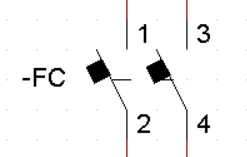
\includegraphics[width=3cm, height=3cm]{Device/AutomaticSwitchII.png}}  & \raisebox{-\totalheight}{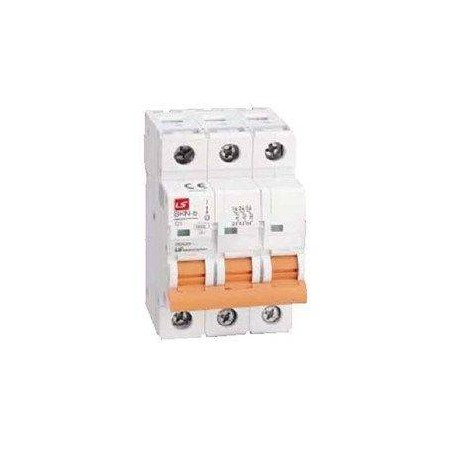
\includegraphics[width=3cm, height=3cm]{Device/AutomaticSwitchII.jpg}}  \\ \hline
  \cellcolor[HTML]{A6637E}{\color[HTML]{FFFFFF} 2}                                 & Automatic Switch IN  & hola & \raisebox{-\totalheight}{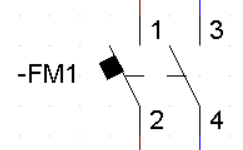
\includegraphics[width=3cm, height=3cm]{Device/AutomaticSwitchIN.png}}  & \raisebox{-\totalheight}{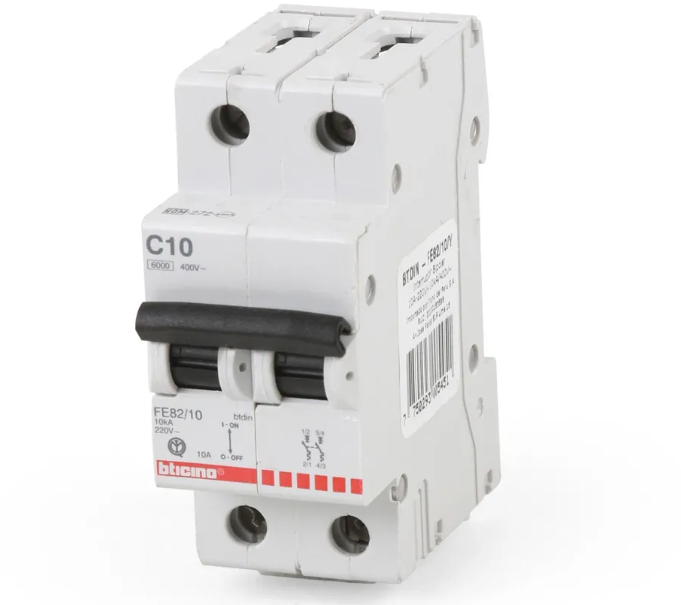
\includegraphics[width=3cm, height=3cm]{Device/AutomaticSwitchINReal.png}}  \\ \hline
  \cellcolor[HTML]{A6637E}{\color[HTML]{FFFFFF} 3}                                 & Coil contactor relay & - & \raisebox{-\totalheight}{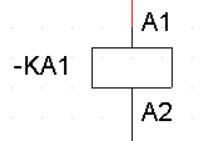
\includegraphics[width=3cm, height=3cm]{Device/CoilContactorRelay.png}} & \raisebox{-\totalheight}{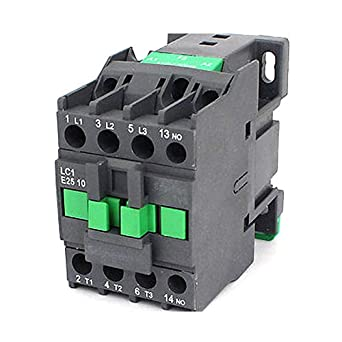
\includegraphics[width=3cm, height=3cm]{Device/CoilContactorRelayReal.jpg}} \\ \hline
  \cellcolor[HTML]{A6637E}{\color[HTML]{FFFFFF} 4}                                 & Contactor III        & - & \raisebox{-\totalheight}{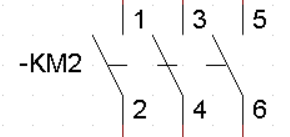
\includegraphics[width=3cm, height=3cm]{Device/ContactorIII.png}}       & ContactorIII       \\ \hline
  \cellcolor[HTML]{A6637E}{\color[HTML]{FFFFFF} 5}                                 & Double Interruptor   & - & \raisebox{-\totalheight}{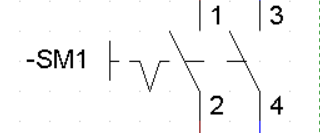
\includegraphics[width=3cm, height=3cm]{Device/doubleInterruptor.png}}  & doubleInterruptor  \\ \hline
  {\color[HTML]{FFFFFF} 6}                                                         & Fuse III             & - & \raisebox{-\totalheight}{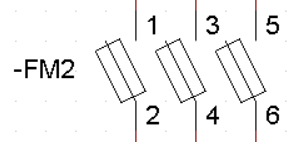
\includegraphics[width=3cm, height=3cm]{Device/FuseIII.png}}            & FuseIII            \\ \hline
  {\color[HTML]{FFFFFF} 7}                                                         & I O II Switch        & - & \raisebox{-\totalheight}{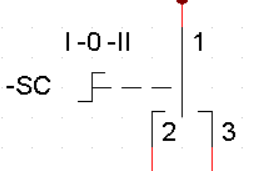
\includegraphics[width=3cm, height=3cm]{Device/I_0_II_Switch.png}}      & I\_0\_II\_Switch   \\ \hline
  {\color[HTML]{FFFFFF} 8}                                                         & Input Conector       & - & \raisebox{-\totalheight}{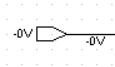
\includegraphics[width=3cm, height=3cm]{Device/inputConection.png}}     & inputConection     \\ \hline
  {\color[HTML]{FFFFFF} 9}                                                         & Mono-Phase Motor     & - & \raisebox{-\totalheight}{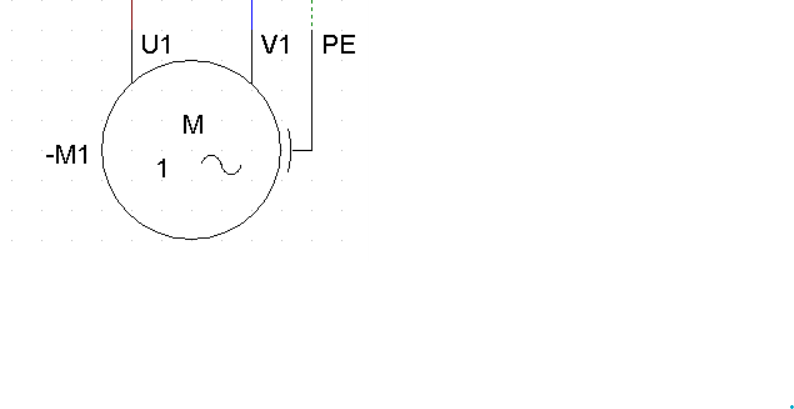
\includegraphics[width=3cm, height=3cm]{Device/monoPhaseMotor.png}}     & monoPhaseMotor     \\ \hline
  {\color[HTML]{FFFFFF} 10}                                                        & N-O Contact          & - & \raisebox{-\totalheight}{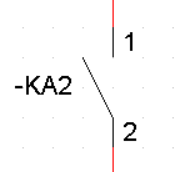
\includegraphics[width=3cm, height=3cm]{Device/NO_Contact.png}}         & NO\_Contact        \\ \hline
  {\color[HTML]{FFFFFF} 11}                                                        & Output Conector      & - & \raisebox{-\totalheight}{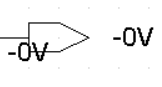
\includegraphics[width=3cm, height=3cm]{Device/outputConector.png}}     & outputConector     \\ \hline
  {\color[HTML]{FFFFFF} 12}                                                        & Pilot Signal         & - & \raisebox{-\totalheight}{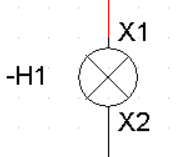
\includegraphics[width=3cm, height=3cm]{Device/PilotSignal.png}}        & PilotSignal        \\ \hline
  {\color[HTML]{FFFFFF} 13}                                                        & Power supply         & - & \raisebox{-\totalheight}{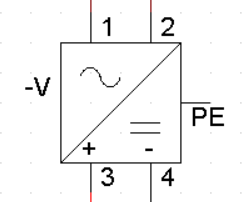
\includegraphics[width=3cm, height=3cm]{Device/powerSupply.png}}        & powerSupply        \\ \hline
  {\color[HTML]{FFFFFF} 14}                                                        & Push button          & - & \raisebox{-\totalheight}{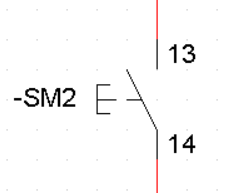
\includegraphics[width=3cm, height=3cm]{Device/pushbutton.png}}         & pushbutton         \\ \hline
  {\color[HTML]{FFFFFF} 15}                                                        & Three phase motor    & - & \raisebox{-\totalheight}{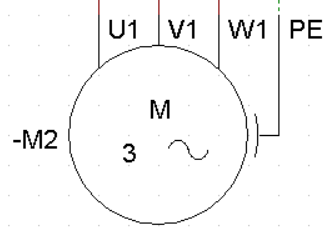
\includegraphics[width=3cm, height=3cm]{Device/ThreePhaseMotor.png}}    & ThreePhaseMotor    \\ \hline
\end{longtable}